\problemname{Minenbeben}
\illustration{.4}{img/Goodluck_Mine.jpg}{%
  \emph{Goodluck Mine, Passage} von Ashley Dace. 
  Lizenz CC BY-SA 2.0.}

\noindent
Die völlig autonomen Mikrobrauereien in den verlassenen Zwergenminen von Moravia sind ein wahres Zeugnis für den Einfallsreichtum und die Handwerkskunst der Zwerge!
Leider werden die Minen manchmal von Erdbeben erschüttert, was dazu führt, dass Rohre und Trichter nicht mehr richtig ausgerichtet sind und kostbare Flüssigkeit auf dem Boden verschüttet wird.
Als erhabener Wächter der Brauereisicherheit ist es deine Aufgabe, die Maschinen in jeder Halle im Falle eines Erdbebens abzuschalten.

Der Gang durch die Tunnel kostet Zeit, 
daher wirst du unweigerlich zu spät an vielen der Maschinen ankommen.
Das lässt sich nicht vermeiden, aber du willst die Gesamtmenge der verschütteten Flüssigkeit so gering wie möglich halten.

\medskip
Die Zwergenminen bestehen aus $n$~Hallen, die durch $n-1$~Tunnel miteinander verbunden sind.
Das gesamte System ist miteinander verbunden, sodass es möglich ist, von jeder Halle zu jeder anderen zu gelangen.
Für die Durchquerung eines Tunnels benötigt man $1$~Zeiteinheit.
Das Ausschalten einer Maschine und das Durchqueren einer Halle nimmt keine Zeit in Anspruch.
In jeder Halle werden, wenn die Maschine zum Zeitpunkt~$t$ nach dem Erdbeben ausgeschaltet wird, insgesamt $t$~Liter Flüssigkeit verschüttet.
Es gibt genau ein Erdbeben, das Erdbeben wirkt sich auf alle Hallen gleichzeitig aus, und du darfst keine Maschine vor dem Erdbeben abschalten.
Du darfst in einer beliebigen Halle beginnen.

\section*{Beispiel}

In Beispieleingabe~$1$ sehen die Minen wie folgt aus:

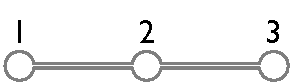
\includegraphics[width=.2\textwidth]{img/sample-1.pdf}

Wenn du in Halle~$2$ beginnst und die restlichen Hallen in der Reihenfolge $2$, $1$, $2$, $3$ besuchst, dann kannst du ihre Maschinen zur Zeit~$0$ (in Halle $2$), zur Zeit~$1$ (in Halle $1$) und zur Zeit~$3$ (in Halle $3$) ausschalten.
Dadurch werden insgesamt $0+1+3=4$~Liter Flüssigkeit verschüttet.
Wenn man stattdessen in Halle~$1$ beginnt und die Hallen in der Reihenfolge $1$, $2$, $3$ besucht, beträgt die Gesamtmenge der verschütteten Flüssigkeit $0+1+2=3$~Liter, was besser ist.

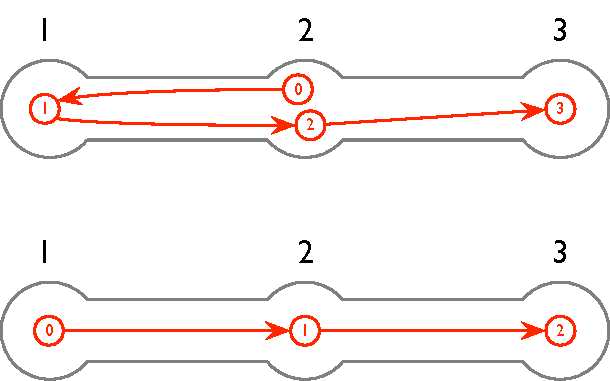
\includegraphics[width=.4\textwidth]{img/sample-1-ans.pdf}

\section*{Eingabe}

Die erste Zeile der Eingabe besteht aus der ganzen Zahl $n$, die die Anzahl der Hallen angibt.
Wir nehmen an, dass die Hallen von $1$ bis $n$ nummeriert sind.
Die nächsten $n-1$ Zeilen enthalten jeweils zwei durch Leerzeichen getrennte ganze Zahlen $u$ und $v$ mit 
$1\leq u < v \leq n$, % constraint:hallnames
was bedeutet, dass es einen Tunnel zwischen Halle~$u$ und Halle~$v$ gibt.

\section*{Ausgabe}

Gibt eine einzelne ganze Zahl aus: die Mindestmenge der verschütteten Flüssigkeit in Litern.

\section*{Beschränkungen und Bewertung}

Es gilt immer
$1\leq n\leq 10^5$. % constraint:n

Deine Lösung wird an einer Reihe von Testgruppen getestet, von denen jede eine bestimmte Anzahl von Punkten wert ist.
Jede Testgruppe enthält eine Reihe von Testfällen.
Um die Punkte für eine Testgruppe zu erhalten, musst du alle Testfälle in der Testgruppe lösen.
Deine endgültige Punktzahl ist die maximale Punktzahl für eine einzelne Einsendung.

\medskip
\begin{tabular}{lll}
Gruppe & Punkte & Beschränkungen \\\hline
  $1$ & $18$ & Keine Halle hat mehr als zwei Tunnel.\\
  $2$ & $19$ & Höchstens eine Halle verfügt über mehr als zwei Tunnel.\\
  $3$ & $20$ & $n\leq 10$\\
  $4$ & $21$ & $n\leq 1000$\\
  $5$ & $22$ & \emph{Keine weiteren Beschränkungen}
\end{tabular}
